After developing and analyzing the different \acs{IoT} system components, it is time to evaluate its overall performance in a real-world scenario. In this chapter, the results of the hospital trial are presented and discussed. 

\section{Hospital Pilot}

For the hospital trial, the proposed \acs{IoT} system was deployed in an clinical facility within Centro Hospitalar e Universitário de Coimbra (CHUC), during which two volunteers were continuously monitoring using the system.

\begin{figure}[H]
    \centering
    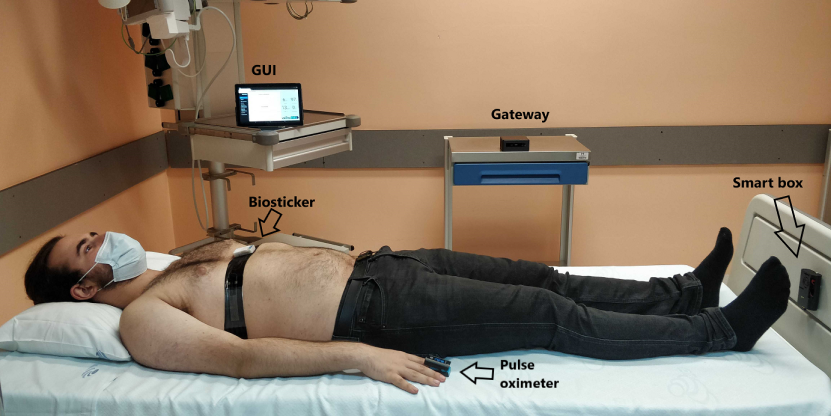
\includegraphics[width=\linewidth]{images/hospital-trial.png}
    \caption[Conceptual illustration of the system components within a medical facility.]{Conceptual illustration of the system components within a medical facility.}
    \label{fig:hospital-trial}
\end{figure}
\dots

To evaluate the performance of the proposed system, the following key performance indicators were defined and measured throughout the tests:

\begin{itemize}
    \item \acs{MQTT} bandwidth -- ;
    \item \acs{FHIR} bandwidth;
    \item \acs{MQTT} latency -- Time difference between the data collection at \textit{SmartBox} and ;
    % \item \acs{MQTT} packet loss -- ;
   
    % \item \acs{FHIR} latency -- Time difference between the data collection at ;
    \item Resource usage of \textit{Gateway} services -- CPU and RAM usage of each \textit{Gateway} service;
\end{itemize}

In the next section, 2 hours of the monitorization are analyzed and discussed. 

\subsection{Results and Discussion}

\begin{figure}[H]
    \centering
    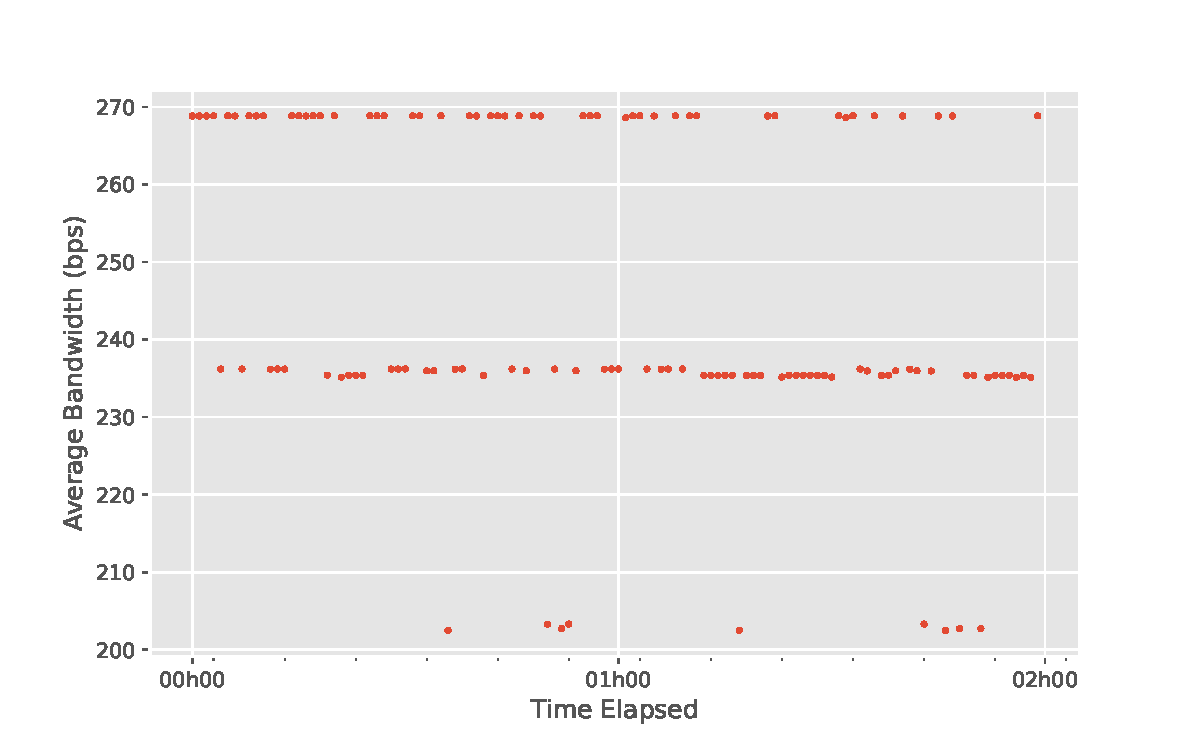
\includegraphics[width=0.66\linewidth]{images/PILOTfhir_bandwidth.pdf}
    \caption{Average \acs{FHIR} usage measured over time.}
    \label{fig:pilot-fhir-bandwidth}
\end{figure}

\begin{figure}[H]
    \centering
    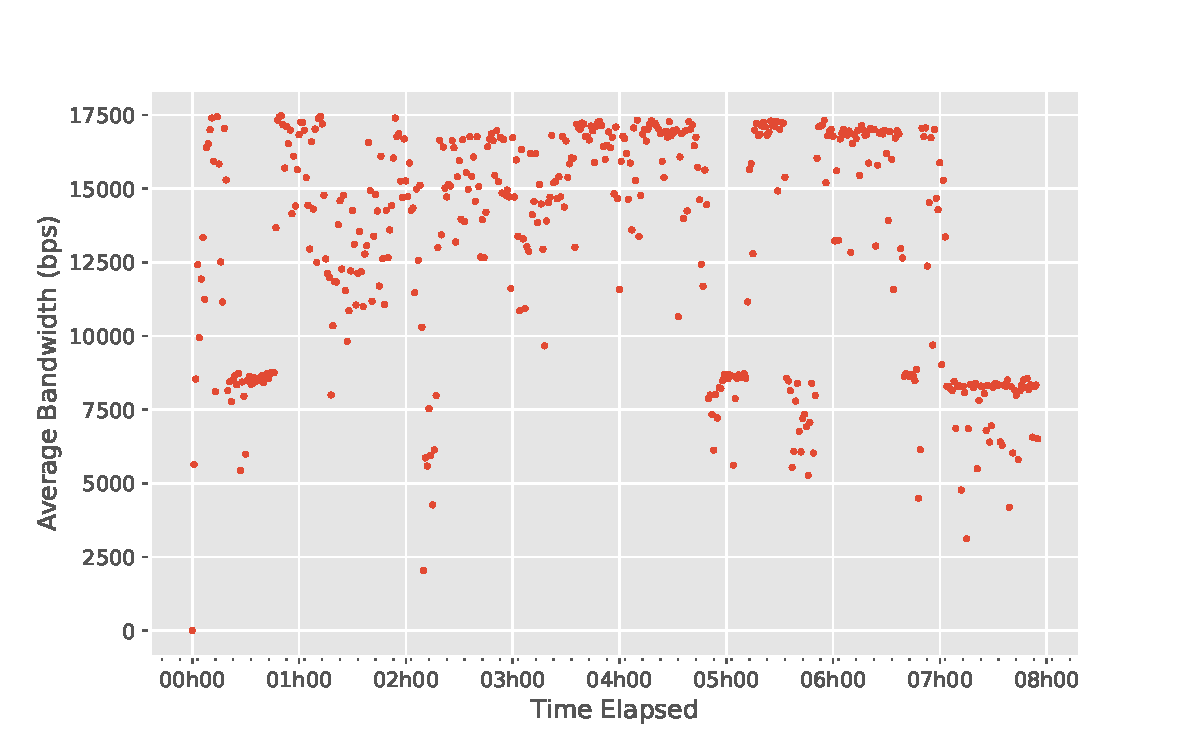
\includegraphics[width=0.66\linewidth]{images/PILOTmqtt_bandwidth.pdf}
    \caption{Average \acs{MQTT} usage measured over time.}
    \label{fig:pilot-mqtt-bandwidth}
\end{figure}

\begin{figure}[H]
    \centering
    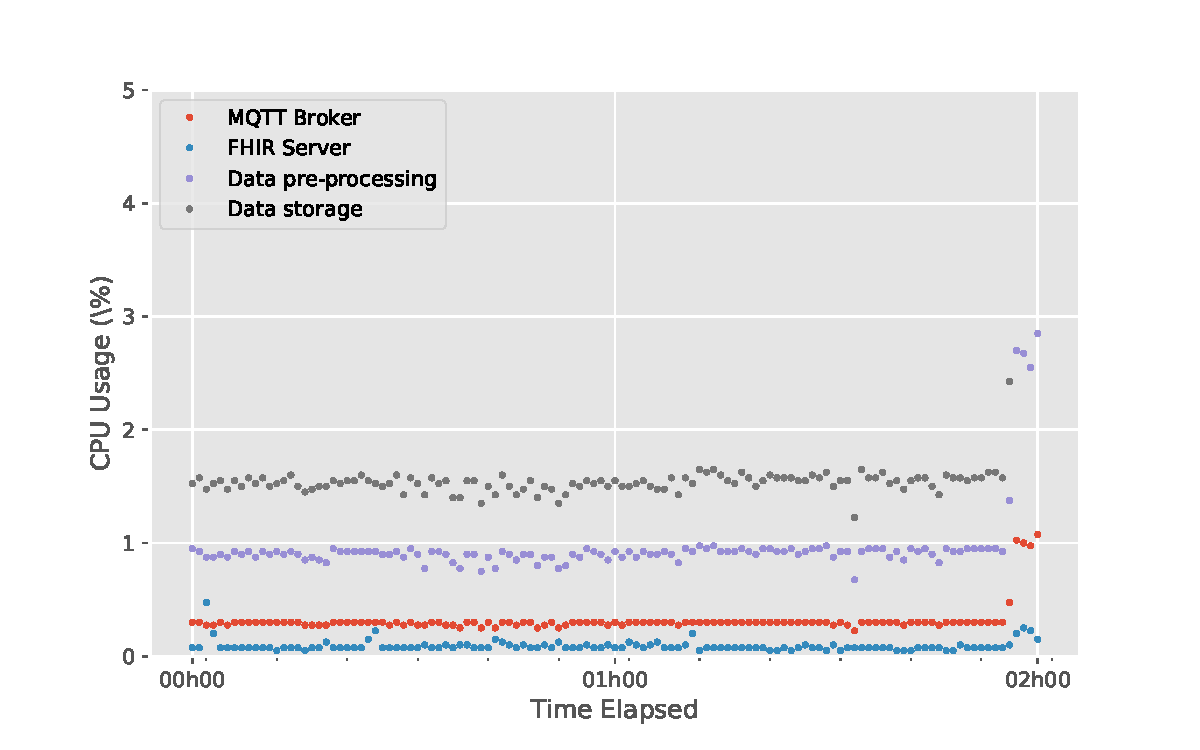
\includegraphics[width=0.66\linewidth]{images/PILOTcpu_usage.pdf}
    \caption{Average CPU usage measured over time.}
    \label{fig:pilot-cou-usage}
\end{figure}

\begin{figure}[H]
    \centering
    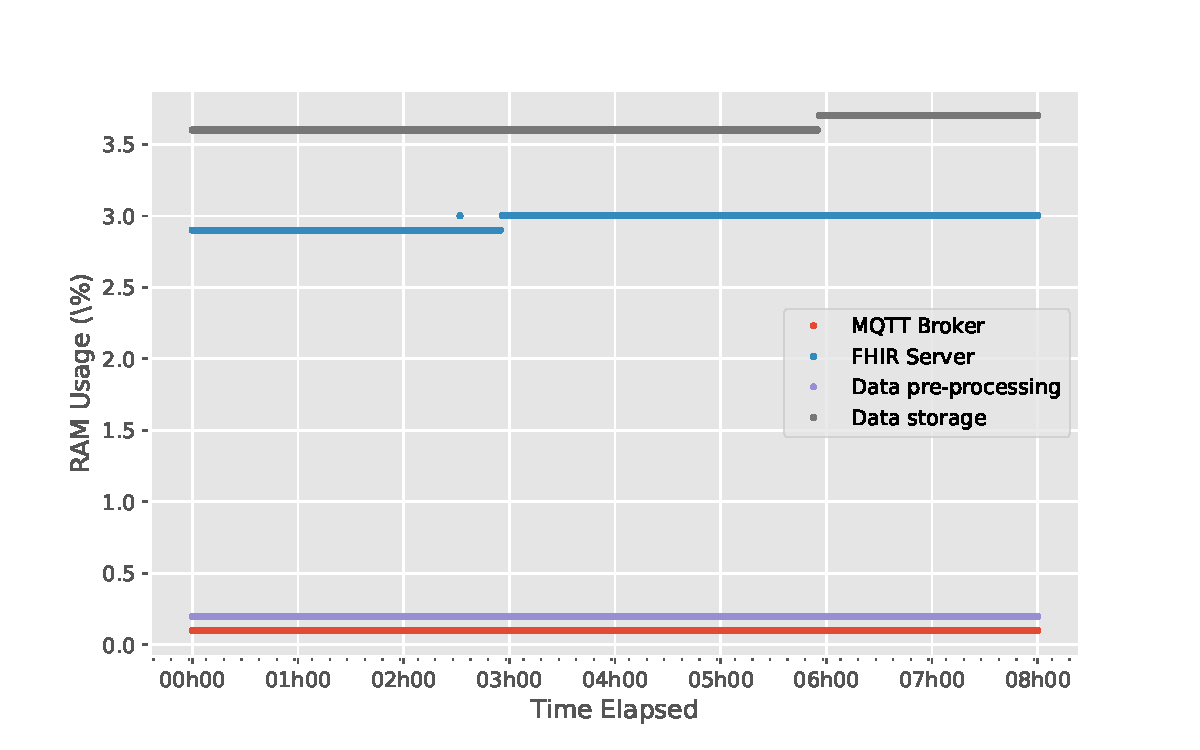
\includegraphics[width=0.66\linewidth]{images/PILOTram_usage.pdf}
    \caption{Average RAM usage measured over time.}
    \label{fig:pilot-ram-usage}
\end{figure}


Network footnote \footnote{https://ubuntu.com/server/docs/network-ntp}

\section{Laboratory Tests}

To evaluate the performance of the proposed system, the following key performance indicators were defined and measured throughout the tests:

\begin{itemize} 
    \item \acs{MQTT} bandwidth --;
    \item \acs{MQTT} latency -- Time difference between the data collection at \textit{SmartBox} and ;
    \item \acs{MQTT} packet loss -- ;
    \item Resource usage of \textit{Gateway} services -- CPU and RAM usage of each \textit{Gateway} service;
\end{itemize}



\section{Summary}
In this chapter, the performance of the proposed system during the hospital trial was tested and discussed. 
In the next, and final chapter, an overview of the work achieved is presented in light of the proposed contributions, concluding with some final remarks.